\chapter{Grundlagen}\label{s:grundlagen}

\section{Stumpfk\"orperaerodynamik (TG)}

%	Stumpfkörper
%	D-Stumpfkörper
%	Strömungsfeld
%	Ablösung
%	Totwasser
%	Wirbelschichten
%	Nachlauf
%	Praktische Bedeutung
%	Ggf. Vergleich schlanke Körper

Im folgenden Kapitel wird der Begriff der Stumpfk"orper in Abgrenzung zu den schlanken K"orpern eingef"uhrt. Eine klare Abgrenzung von schlanken K"orpern zu Stumpfk"orpern bereitet Schwierigkeiten, da der "Ubergang oftmals flie\ss{}end ist. Jedoch unterscheidet sich das Str"omungsbild markant, weswegen im folgenden Kapitel im Besonderen auf das Str"omungsfeld und die Charakteristiken des Nachlaufs eingegangen werden sollen.

\subsection{Geometrische Einordnung}
\label{sec:Geometrie}
Ein stumpfer K"orper in einer Anstr"omung differenziert sich geometrisch von einem schlanken insofern, dass er eine signifikante Dicke quer zur Anstr"omung aufweist, welche in vergleichbarer Gr"o\ss{}enordnung wie die Abmessungen parallel zur Anstr"omung liegt. Als Ma\ss{} kann das Dickenverh"altnis $\sigma$ als Kehrwert des Schlankheitsgrades $\lambda$ herangezogen werden, welches das Verh"altnis von Dicke zu Breite wiedergibt:

\begin{align}
\sigma = \frac{1}{\lambda} = \frac{d}{l}
\end{align}

Wie in \abb{fig:HuchoDV} zu sehen ist, ver"andert sich das Str"omungsbild ma\ss{}geblich mit steigendem Dickenverh"altnis $\sigma$, wobei der "Ubergang von schlanken K"orpern ($\sigma = 0,13$) zu stumpfen K"orpern ($\sigma = 0,5$) flie\ss{}end ist.

\begin{figure}[h]
	\centering
	\begin{subfigure}[c]{0.45\textwidth}		
		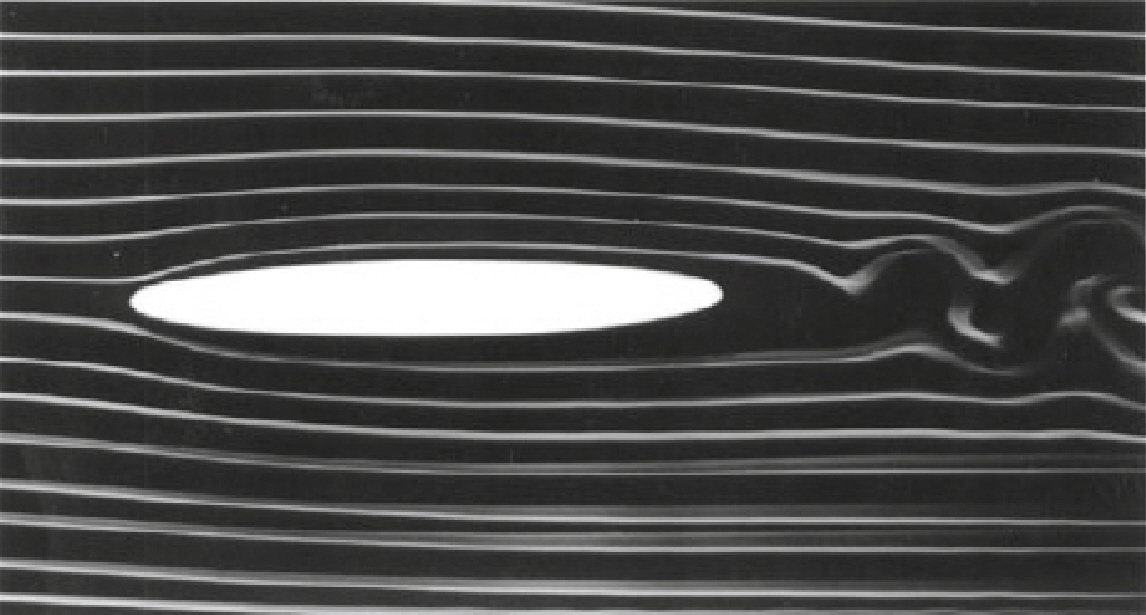
\includegraphics[width=1\textwidth]{HuchoDV013.jpg}
		\subcaption{$\sigma = 0,13$}
	\end{subfigure}
	\begin{subfigure}[c]{0.45\textwidth}
		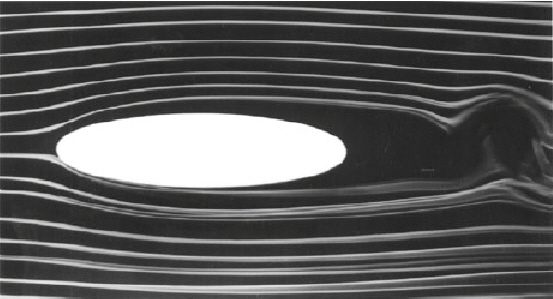
\includegraphics[width=1\textwidth]{HuchoDV026.jpg}
		\subcaption{$\sigma = 0,26$}
	\end{subfigure}
	\begin{subfigure}[c]{0.45\textwidth}
		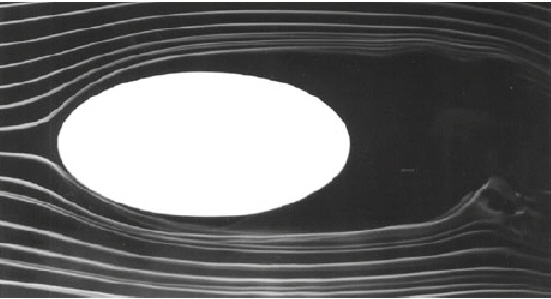
\includegraphics[width=1\textwidth]{HuchoDV05.jpg}
		\subcaption{$\sigma = 0,5$}
	\end{subfigure}
	\caption{elliptische Zylinder unterschiedlicher Dickenverh"altnisse im Rauchkanal \cite{Hucho.2011}}
	\label{fig:HuchoDV}
\end{figure}


Obwohl das Dickenverh"altnis in allgemeiner N"aherung ein gutes Ma\ss{} f"ur die Einordnung eines Stumpfk"orpers ist, zeigt sich in der Praxis, dass es nicht als notwendiges Kriterium herangezogen werden kann. So treten vergleichbare Effekte der Stumpfk"orperaerodynamik ebenfalls bei einem diskontinuierlichen Verlauf der K"orpergeometrie auf. Dies ist beispielsweise bei der ausgepr"agten Hinterkanten eines Fahrzeughecks der Fall. Der Verlauf der K"orpergeometrie muss also ebenfalls als geometrische Charakterisierung eines stumpfen K"orpers herangezogen werden.


\subsection{Str"omungsbild}
\label{sec:Stromungsbild}
Bei der Umstr"omung eines K"orpers kommt es aufgrund der Haftbedingung an dessen Kontur zur Ausbildung einer Grenzschicht. W"ahrend die Str"omungsgeschwindigkeit an der K"orperoberfl"ache Null betr"agt, passt sie sich im Grenzschichtbereich an die Anstr"omgeschwindigkeit an. Ein Teil der kinetischen Energie der Grenzschichtstr"omung wird durch Reibung an der Wand dissipiert.
Die Geometrie eines stumpfen K"orpers, wie in \abb{fig:HuchoDV} dargestellt, f"uhrt bei Umstr"omung gem"a\ss{} Bernoulli zu einer Absenkung des statischen Drucks $p$ bis zur dicksten Stelle. Hinter dieser steigt der statische Druck $p$ wieder an, wobei die durch Reibung verringerte kinetische Energie nicht mehr ausreicht, um gegen diesen anzustr"omen. Ist die kinetische Energie vollends in Druck umgewandelt, kommt es zur R"uckstr"omung, wobei die Grenzschicht abl"ost \cite{Hucho.2011}.\\
Sofern eine diskontinuierlichen Stelle in der K"orpergeometrie vorhanden ist, kann die Str"omung dieser ebenfalls nicht weiter folgen. Man spricht in diesem Fall von einem Abriss der Str"omung, welcher in der Praxis an Hinterkanten zu finden ist.

Das Abl"osen oder Abrei\ss{}en hat die Ausbildung eines Totwassers zur Folge, in dessen Gebiet sich das Fluid bedingt durch Z"ahigkeitseffekte verwirbelt und Wirbelschichten ausbildet. Dies f"uhrt zu einer Druckabsenkung hinter dem stumpfen K"orper, sodass durch den h"oheren Staupunktdruck an der Vorderseite ein Druckgradient zu verzeichnen ist. Ein Druckwiderstand ist die Folge, welcher in Str"oumgsrichtung des Fluides wirkt. Wie man in \abb{fig:HuchoStumpf} sehen kann, ist das Totwasser ein Charakteristikum des Str"omungsbildes stumpfer K"orper. Im Vergleich dazu ist dieses Gebiet beim Str"omungsbild schlanker K"orper, wie in \abb{fig:HuchoSchlank} zu sehen, nicht vorhanden, da hier ein nahezu st"orungsfreies Abstr"omen m"oglich ist. Lediglich die Reibungseffekte innerhalb der Grenzschichtstr"omung sorgen hier f"ur einen Reibungswiderstand. Schluss folglich wird der Gesamtwiderstand bei stumpfen K"orpern vom Druckwiderstand, der bei schlanken K"orpern jedoch vom Reibungswiderstand dominiert.

\begin{figure}[h]
	\centering
	\includegraphics[width=0.5\textwidth]{HuchoschlankerKorper.jpg}
	\caption{Stromlinienbild eines schlanken K"orpers im Rauchkanal \cite{Hucho.2011}}
	\label{fig:HuchoSchlank}
\end{figure}

\begin{figure}[h]
	\centering
	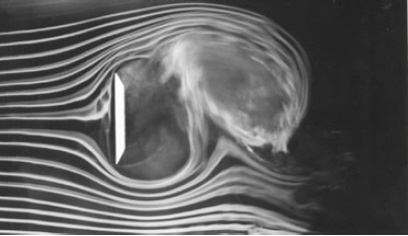
\includegraphics[width=0.5\textwidth]{HuchoStumpferKorper.jpg}
	\caption{Stromlinienbild eines stumpfen K"orpers im Rauchkanal \cite{Hucho.2011}}
	\label{fig:HuchoStumpf}
\end{figure}


Hieraus wird die Notwendigkeit ersichtlich, eine Druckerh"ohung in diesem Totwasser vorzunehmen, um den Druckgadienten und damit den Druckwiderstand zu verringern. F"ur das bessere Verst"andnis soll im nachfolgenden das Totwasser weiter spezifiziert werden.

\subsection{Totwasser}
\label{sec:Totwasser}

Wie bereits oben erw"ahnt bilden sich innerhalb des Totwassers Wirbelschichten aus. Diese entstehen bei der turbulenten Durchmischung der ehemaligen Grenzschichtstr"omung, welche nun als Scherschichtstr"omung bezeichnet wird, mit dem ruhenden Fluid im Windschatten des K"orpers. 



 
Innerhalb des Totwassers existiert eine instation"are periodische Str"omung, welche durch Druckschwankungen zu oszillierende Abl"osungen f"uhrt. Diese Oszillation wei\ss{}t eine charakteristische Frequenz auf und wird durch die Stouhal-Zahl ${Sr}$ beschrieben. 

Die Wirbel innerhalb der turbulenten Str"omung  zerfallen kaskadenartig in kleinere Wirbel und dissipieren dabei ihre Energie in W"arme, bis sie sich g"anzlich aufl"osen und sich erneut ein laminares Str"omungsprofil ausbildet. Dennoch ergibt sich im Nachlauf des stumpfen K"orpers eine Delle im Geschwindigkeitsfeld. 

\begin{figure}[h]
	\centering
	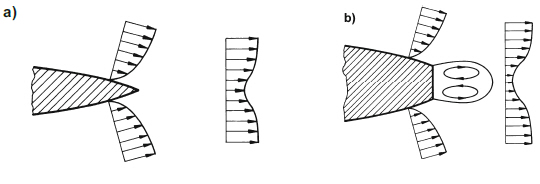
\includegraphics[width=0.7\textwidth]{Nachlauf.jpg}
	\caption{Nachlauf eines a) schlanken K"orpers und eines b) stumpfen K"orpers \cite{Hucho.2011}}
	\label{fig:Nachlauf}
\end{figure}

\subsection{Praktische Bedeutung der Stumpfk"orper}
tbd


\section{Coand\^{a}-Effekt (TG)}
%	Umströmung gekrümmter Flächen
%	Haftbedingung
%	Typische Strömungsbilder
%	technische Anwendung 

Der Coand\^{a}-Effekt tritt auf, wenn ein Strahl entlang einer konvexen K"orperkontur str"omt. Anders als die bisher betrachtete Str"omung, kann die sogenannte Coand\^{a}-Str"omung des Strahles der Kontur einer konvexen Rundung folgen ohne abzul"osen, wie dies in \abb{fig:coanda} deutlich wird. Dem Gegen"uber f"uhrt die konvexe Rundung bei einer normalen Anstr"omung nach Bernoulli zu einer Verlangsamung der Str"omung und demgem"a\ss{} einer Druckerh"ohung, was eine R"uckstr"omung und Abl"osung zur Folge hat. Dies wurde bereits in \ref{sec:Stromungsbild} diskutiert.

\begin{figure}[h]
	\centering
	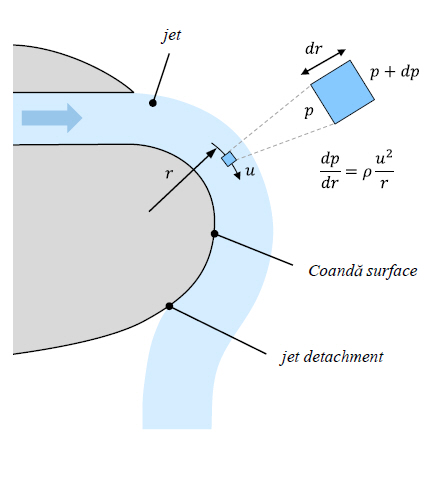
\includegraphics[width=0.5\textwidth]{coanda.jpg}
	\caption{Skizze zum Coand\^{a}-Effekt \cite{Stadlberger.2016}}
	\label{fig:coanda}
\end{figure}

Tritt ein Freistrahl in ein ruhendes Fluid ein, rei\ss{}t er an dessen R"andern das umgebende Medium mit. Um die Kontinuit"atsbedingung zu erf"ullen, entsteht am Au\ss{}enraum des Strahls eine Str"omung zur Strahlmitte, was als Entrainment-Effekt bezeichnet wird. In der N"ahe einer K"orperkontur wird das Nachstr"omen des Mediums unterbunden wird. In der Folge entsteht an der Wand ein lokaler Unterdruck und somit ein Druckgradient $dp$ quer zur Str"omungsrichtung. Dies f"uhrt zu einer Umlenkung des Freistahl in Richtung der Wand, wie in \abb{fig:coanda} ersichtlich ist. In der Folge entsteht ein Wandstrahl, welcher sich an die K"orperkontur anschmiegt \cite{Fernholz.1966}. 

Die Kr"ummung pr"agt dem Strahl eine Zentrifugalkraft auf, welche im Gleichgewicht mit der Resultierenden infolge des Druckgradienten $dp$ steht. Eine Erh"ohung der Wandkr"ummung ruft jedoch eine st"arkere Zentrifugalkraft hervor. Deshalb kann der Wandstrahl starken Kr"ummungen durch kleine Wandradien nicht folgen und l"ost ebenfalls ab \cite{Riedel.1971}

%Ausführung Riedel ergänzen
Da es sich bei der Coand\^{a}-Str"omung um einen Wandstrahl handelt, gibt es zur Grenzschicht eine zus"atzliche Reibungsschicht zum umgebenden Medium. Somit bildet sich ein Geschwindigkeitsprofil wie in \abb{fig:Wandstrahl} aus. \\

\begin{figure}[h]
	\centering
	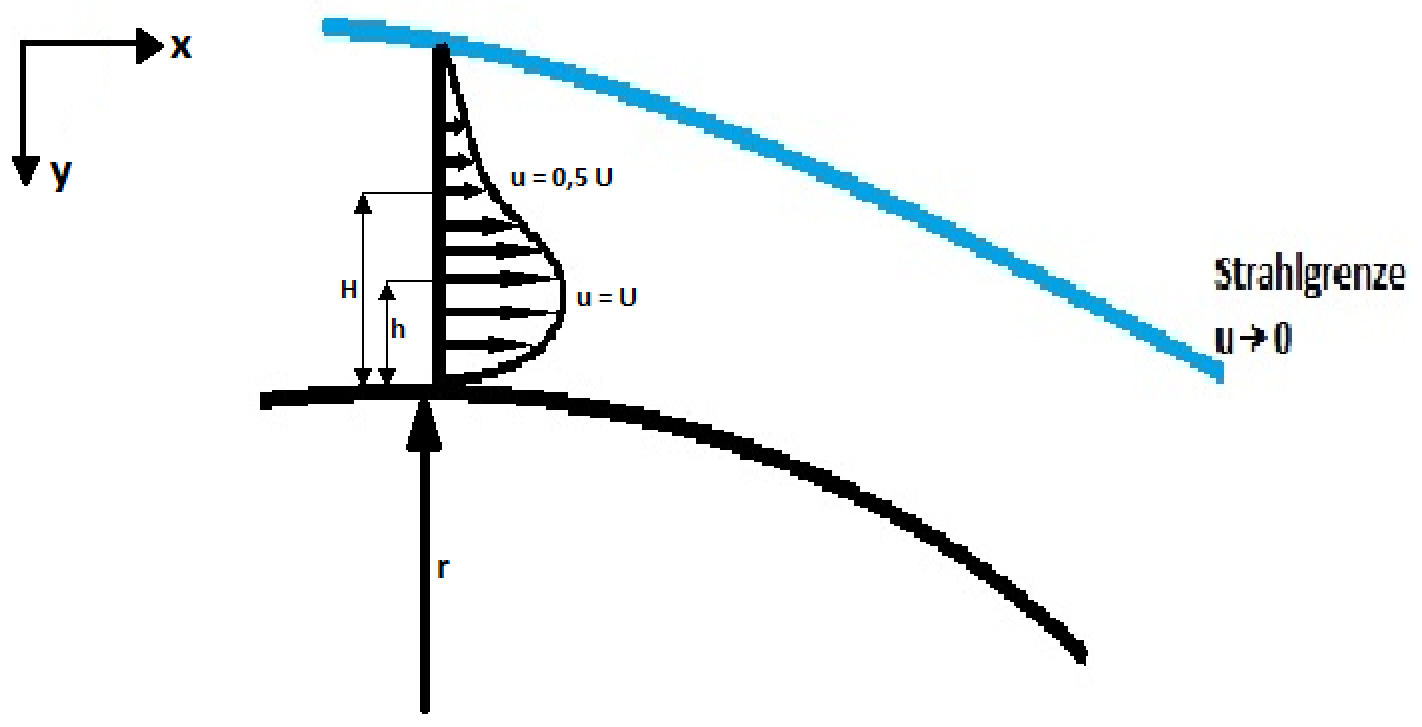
\includegraphics[width=0.9\textwidth]{Wandstrahl.jpg}
	\caption{Geschwindigkeitsprofils eines Wandstrahls an einer konvexen K"orperkontur nach Riedel \cite{Riedel.1973}}
	\label{fig:Wandstrahl}
\end{figure}

Im zeitlichen Mittel ist die resultierende Zentrifugalkraft proportional zu $\frac{u^2}{r+y}$. Dabei ist die wirkende Zentrifugalkraft in der N"ahe des Maximums des Geschwindigkeitsprofils des Wandstrahls proportional zu $\frac{U^2}{r+\frac{H}{4}}$. Sie ist somit aufgrund der h"oheren Geschwindigkeit gr"o\ss{}er als die Zentrifugalkraft auf Teilchen in der N"ahe der Strahloberfl"ache und in der N"ahe der K"orperkontur.\\
An der K"orperkontur ist die resultierende Zentrifugalkraft proportional zu $\frac{u^2}{r}$, an der Strahloberfl"ache jedoch nur zu $\frac{0,25 \cdot U^2}{r + H}$. Aus diesem Grund besteht die Tendenz von Teilchen in der N"ahe der Maximalgeschwindigkeit, zum "au\ss{}eren Rand und somit in das Gebiet der Strahlvermischung mit dem Umgebungsmedium abzudriften. Durch ihre geringere Zentrifugalkraft blockieren die Teilchen innerhalb des "au\ss{}eren Randes jedoch die nach au\ss{}en dringenden Teilchen und somit eine nach au\ss{}en gerichtete Bewegung. Infolgedessen treffen zus"atzliche Teilchen am Rand aufeinander, was feine Strahlvermischung bef"ordert.\\
Ein entgegengesetztes Verhalten findet sich in der N"ahe der K"orperkontur. Den Teilchen in Wandn"ahe wird eine kleinere Zentrifugalkraft als im Strahlzentrum aufgepr"agt. Weniger Kollisionen und somit eine geringere gegenseitige Beeinflussung benachbarter Teilchen sind die Folge. Dies reduziert den Turbulenzgrad verglichen mit einer ebenen Strahlstr"omung.
Stromabw"arts weitet sich die Mischbewegung vom Strahlrand zum Strahlkern und zur konturnahen Str"omung aus, weshalb der Turbulenzgrad infolge der Strahlvermischung steigt \cite{Riedel.1973}. 

Wie bereits oben erw"ahnt wurde, wird am freien Rand das umgebende Fluid mitgerissen, was gleichzeitig zu einer Reduktion der kinetischen Energie des Strahls f"uhrt. Die daraus resultierende Verlangsamung der Coand\^{a}-Str"omung sorgt daf"ur, dass die Abl"oseneigung des Strahls mit der Laufl"ange zunimmt \cite{Fischer.2011}. Aus dieser Beobachtung heraus wurde der Anlegewinkel f"ur Coand\^{a}-Str"omung an einem Zylinder durch Newman definiert \cite{Newman.1961}. Dieser beschreibt das Verh"altnis vom Radius $R$ der konvexen K"orperkontur zur Ausdehnung $h$ des Strahls. Die Ausdehnung $h$ des Strahls wird durch die Spalth"ohe bestimmt, weshalb der Anlegewinkel eine fundamentale Beziehung geometrisch signifikanter Gr"o\ss{}en der Coand\^{a}-Fl"achen-Ausblasung beschreibt. Infolge h"oherer Zentrifugalkr"afte bei gro\ss{}en Wandkr"ummungen nimmt der Anlegewinkel bei kleinen $\frac{h}{R}$ und konstanten Ausblasimpuls zu. Wird die Spalth"ohe kleiner, erh"oht sich gem"a\ss{} der Kontinuit"atsgleichung die Ausblasgeschwindigkeit. Diese Geschwindigkeiterh"ohung sorgt f"ur eine Effektivierung des Entrainment-Effektes und in Folge dessen ebenfalls der Coand\^{a}-Effekt \cite{Fischer.2011}.


%%
%Da es sich bei der Coand\^{a}-Str"omung um einen Wandstrahl handelt, gibt es zur Grenzschicht eine zus"atzliche Reibungsschicht zum umgebenden Medium. Dies wird in \abb{fig:coanda} gezeigt. Da das Umgebungsmedium ruht, gibt es gem"a\ss{} Bernoulli keinen Druckanstieg entlang der konvexen Rundung, die Grenzschicht bleibt stabil. Aus diesem Grund haftet die Coand\^{a}-Str"omung l"anger an K"orperkontur an.




%%%%%%%%%%%%%%%%%%%%%%%%%%%%%%%%NORAS REICH ;) %%%%%%%%%%%%%%%%%%%%%%%%%%%%%%%%%%%%%%%%%%%%%%%%%
\newpage
\section{Aktive Str\"omungsbeeinflussung (NB)}

Stumpfe K"orper haben meist ein stufenartiges Ende, an dem sich str"omungsmechanische Nachteile ergeben. Deshalb soll durch eine Anpassung der Geometrie des K"orpers oder durch die strukturelle Ver"anderung des Todwassers dieser ausgeglichen werden. Ziel ist es, den Basisdruck anzuheben und dar"uber den Druckwiderstand des K"orpers zu verringern \cite{Hucho.2011}.\\
%hier evtl ein paar passive verfahren
Die nachfolgende Arbeit konzentriert sich auf ein aktives Verfahren der Str"omungsbeeinflussung, weshalb im folgenden einige bis jetzt realisierte Verfahren vorgestellt werden.\\

%-------------------------------------------------------------------------------------
Bearman \cite{Hucho.2011} hat als einer der ersten die aktive Str"omungsbeeinflussung nachgewiesen. \abb{fig:Bearman} zeigt das verwendete Stumpfk"orpermodell. Dabei ist als Besonderheit auf die por"ose Basis \(A_{0}\) hinzuweisen, durch die zus"atzlich Luft am Ende des K"orpers ausgesto\ss{}en wird. Es werden zwei Ausblasequerschnitte \(A_{0}\) gew"ahlt, einmal "uber fast die gesamte Fl"ache und einmal "uber knapp die H"alfte der Fl"ache in der Mitte angeordnet.
\begin{figure}[h]
	\centering
	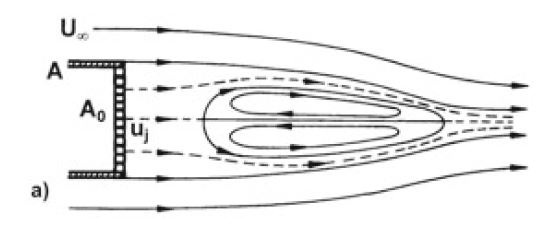
\includegraphics[width=0.5\textwidth]{KorperBearman.jpg}
	\caption{Stumpfk"orper mit Ausblasung von Bearman \cite{Hucho.2011}}
	\label{fig:Bearman}
\end{figure}\\
Der Druck hinter dem K"orper nimmt mit wachsendem Volumenstrom zu. Die austretende Luft sorgt daf"ur, dass die Str"omungsabl"osung vom K"orperende weggeschoben wird. Sie fungiert wie eine Trennplatte im Bereich der passiven Str"omungsbeeinflussung. Durch die erst weiter hinten stattfindende Verwirbelung, f"allt der Widerstand des K"orpers ab.

%-------------------------------------------------------------------------------------
Geropp und Odenthal beschreiben in \cite{Geropp.2000} Experimente zur Einblasung am Ende eines Kraftfahrzeuges "uber zwei Schlitze mit Nutzung des Coand\^{a}-Effekts (\abb{fig:Geropp}).
\begin{figure}[h]
	\centering
	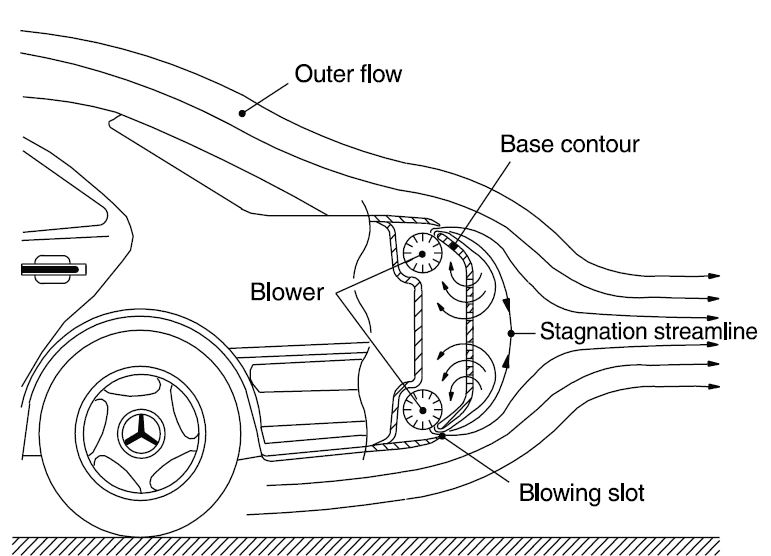
\includegraphics[width=0.5\textwidth]{KorperGeropp.jpg}
	\caption{Stumpfk"orper mit Ausblasung von Geropp \cite{Geropp.2000}}
	\label{fig:Geropp}
\end{figure}\\
Hierbei ist f"ur die Beeinflussung der Grenzschicht die Ausblasung bei hohen Geschwindigkeiten erforderlich. Durch den Coand\^{a}-Effekt wird die eingeblasene Luft in das Todwasser umgelenkt, wo sie wieder abgesaugt wird. Dadurch wird der Druck hinter dem Fahrzeug erh"oht und der Gesamtwiderstand verrringert. Die Experimente zeigen, dass eine Druckerh"ohung von~50\% und eine Widerstandsverringerung um 10\% m"oglich ist. Au\ss{}erdem wird ein Energievorteil f"ur moderate Ausblasgeschwindigkeiten mathematisch festgestellt.

%--------------------------------------------------------------------------------------
In \cite{Barros.2016} wird zus"atzlich zu den vorher beschriebenen Verfahren die Ausblassung gepulst durchgef"uhrt. Dabei soll der Einfluss von Frequenz und Amplitude auf das Widerstandsverhalten untersucht werden.\\
In \abb{fig:Barros} ist der schematische Aufbau der gepulsten Ausblasung dargestellt. Diese wird "uber Ventile realisiert, die eine Rechteckkurve mit einem duty cycle (weitere Erl"auterungen in \kap{s:rotierendeWalzen}) von 40\% erzeugen. Direkt unter der Ausblasstelle wird zus"atzlich noch eine Coand\^{a}-Fl"ache befestigt.\\
\begin{figure}[h]
	\centering
	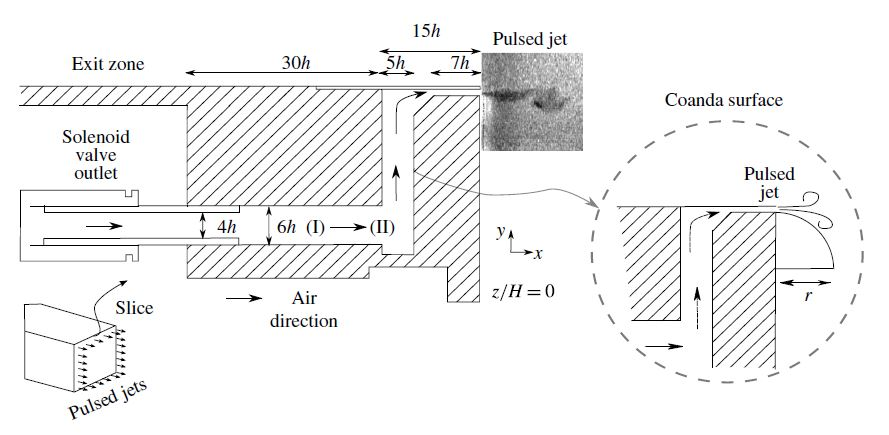
\includegraphics[width=0.7\textwidth]{KorperBarros.jpg}
	\caption{Ausblasung von \cite{Barros.2016}}
	\label{fig:Barros}
\end{figure}
Mit eher steigender Frequenz und steigender Amplitude, wurde eine Umlenkung der Grenzschicht beobachtet. "Uber eine gepulste Einblasung, nahe der nat"urlichen Abl"osefrequenz der Str"omung, kann nach \cite{Barros.2016} der Widerstand am meisten (10\%) gesenkt werden. Bei zus"atzlicher Nutzung der Coand\^{a}-Fl"ache kann eine Reduktion von 20\% erreicht werden.

%-------------------------------------------------------------------------------------
Modi et al. \cite{MODI.1991} versucht durch drehende Zylinder den Widerstand zu reduzieren. Dabei benutzt \cite{MODI.1991} unterschiedliche Modelle. F"ur erste Versuche wird das Modell in \abb{fig:Modi3} benutzt und sp"ater der Truck aus \abb{fig:Modi}.
\begin{figure}[h]
	\centering
	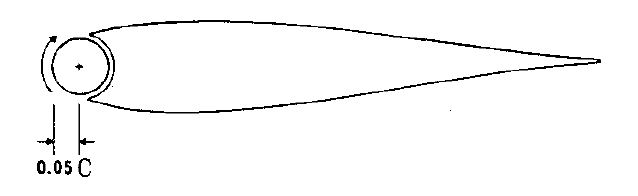
\includegraphics[width=0.6\textwidth]{KoerperModi3.jpg}
	\caption{Stumpfk"orpermodell mit Walze von Modi et al. \cite{MODI.1991}}
	\label{fig:Modi3}
\end{figure}\\
F"ur den K"orper in \abb{fig:Modi3} sind Str"omungsbilder (\abb{fig:ModiStr}) aufgenommen worden. Diese sind mit einem Anstellwinkel des K"orpers von 20 Grad entstanden. Das Verh"altnis der Drehgeschwindigkeit der Zylinder \(U_c\) bzgl. der Anstr"omgeschwindigkeit \(U\) wurde variiert.\\
\begin{figure}[h]
	\centering
	\begin{subfigure}[c]{0.4\textwidth}		
		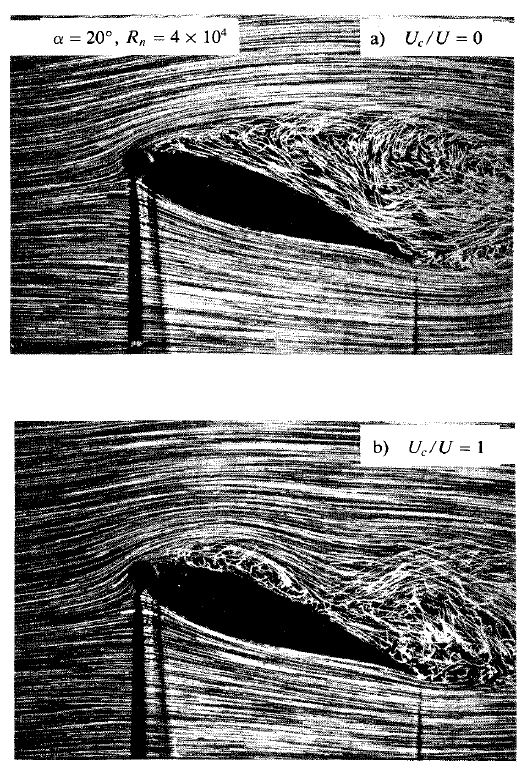
\includegraphics[width=0.7\textwidth]{ModiStr1.jpg}
	\end{subfigure}
	\begin{subfigure}[c]{0.4\textwidth}
		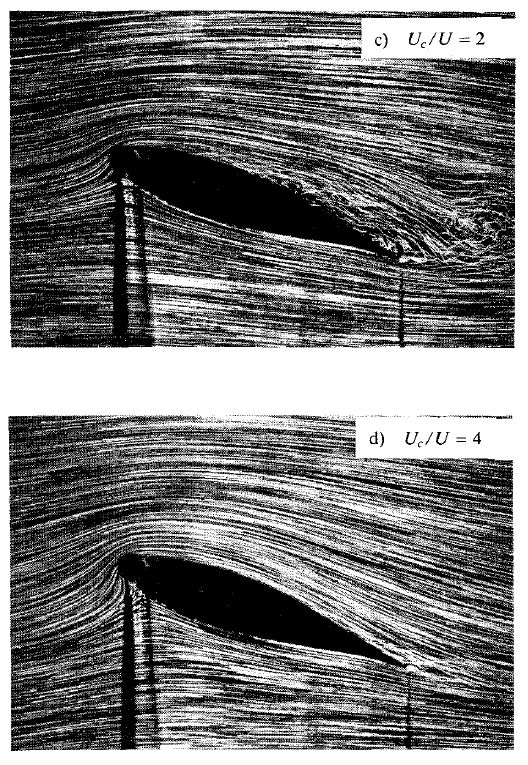
\includegraphics[width=0.7\textwidth]{ModiStr2.jpg}
	\end{subfigure}
	\caption{Str"omungsbilder von Modi et al. \cite{MODI.1991}}
	\label{fig:ModiStr}
\end{figure}

Auf den Str"omungsbildern (\abb{fig:ModiStr}) kann gut gesehen werden, dass bei nicht rotierenden Zylindern \(U_c/U=0\) (oben links) die Abl"osung stark ist im Vergleich zu \(U_c/U=4\) (unten rechts), hier drehen die Zylinder viermal schneller als die Anstr"omung.\\
\begin{figure}[h]
	\centering
	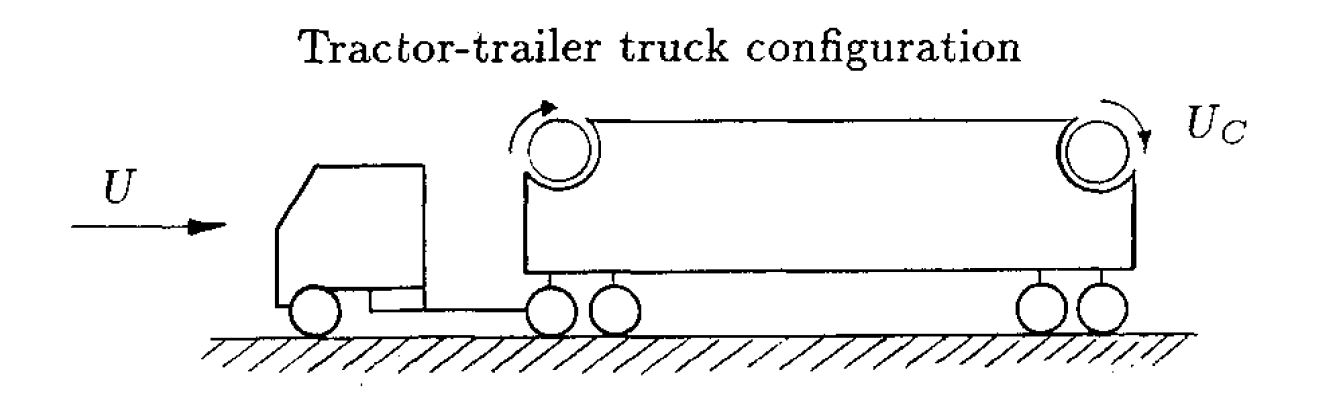
\includegraphics[width=0.6\textwidth]{KorperModi.jpg}
	\caption{Erstes Truckmodell von Modi et al. \cite{MODI.1991}}
	\label{fig:Modi}
\end{figure}
Bei den Versuchen am Truckmodell sind die Zylinder zuerst angeordnet, wie in \abb{fig:Modi} dargestellt. Bei dem ersten Versuch werden die Rauhigkeiten der Zylinder variiert. Es gibt einen glatten Zylinder, einen mit einer Rauhigkeit von 40 und einen mit 80. Au\ss{}erdem wird wieder das Verh"altnis der Drehgeschwindigkeiten der Zylinder \(U_c\) bzgl. der Anstr"omgeschwindigkeit \(U\) f"ur alle drei F"alle variiert. Daraus ergeben sich die Widerstandsreduktionen in \tab{tab:Modi}.\\
\begin{table}[h]
	\centering
	\begin{tabular}{lrr}
		\toprule
		Zylinder & Widerstandsreduktion [\%] & \(U_c/U\)\\
		\midrule
		glatt & 5 & 2\\
		Rauhigkeit 80 & 10 & 2.1\\
		Rauhigkeit 40 & 13 & 2.1\\
		\bottomrule
	\end{tabular}
	\caption{Widerstandsreduktion bei Modi}
	\label{tab:Modi}
\end{table}
Da der hintere Zylinder keinen Impuls in die Grenzschicht einbringen kann, wurde ein zweites Experiment mit anderer Konfiguration durchgef"uhrt. Dabei wurde ein Zylinder mit spiralf"ormiger Rille in der Oberfl"ache und einer mit einer Vielkeil-Verzahnung, deren Rillen parallel zur Drehachse verlaufen, verwendet. Die Position des ersten Zylinders bleibt unver"andert, der Zweite wird ans Ende des ersten Drittels der Truckoberseite positioniert (siehe \abb{fig:Modi2}).\\
\begin{figure}[h]
	\centering
	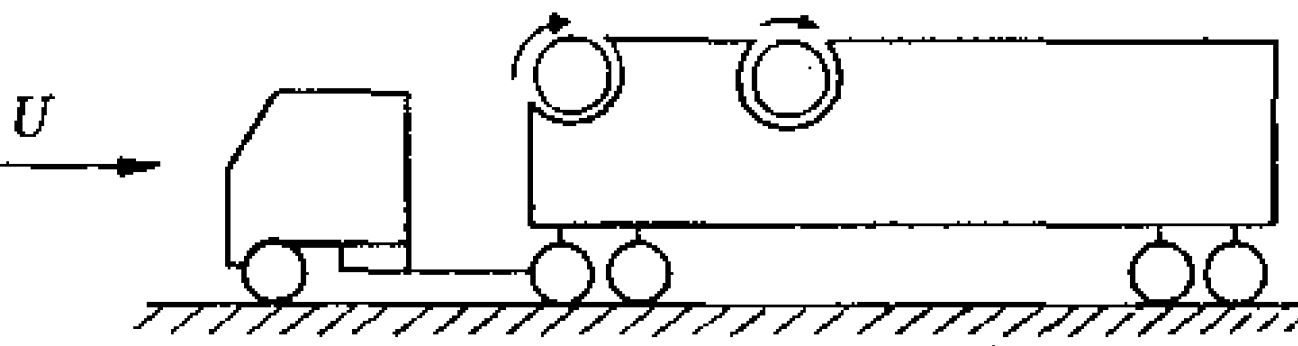
\includegraphics[width=0.5\textwidth]{KoerperModi2.jpg}
	\caption{Zweites Truckmodell von Modi et al. \cite{MODI.1991}}
	\label{fig:Modi2}
\end{figure}\\
Der spiralf"ormige Zylinder erzielte das gleiche Ergebnis, wie der Zylinder mit einer Rauhigkeit von~40 im ersten Experiment. Der Vielkeil-Verzahnungszylinder hat allerdings einen gro\ss{}en Einfluss auf den Widerstand. Bei alleiniger Betrachtung des vorderen Zylinders wird eine Reduktion von~29\% erreicht, beide Zylinder erreichen bis zu 41\%.

%------------------------------------------------------------------------------------
In \cite{Gong.2015} wird eine r"uckwertsgewandte Stufe ein 2D-Modell und anschlie\ss{}end ein 3D-Model (\abb{fig:Gong}) untersucht. Das besondere dabei ist die Anregungsform "uber einen Lautsprecher, der ein monofrequentes, sinusf"ormiges Anregunfgssignal durch kleine L"ocher in die Str"omung gibt. "Uber die Sinusfunktion wird erreicht, dass die eingestr"omte Masse "uber eine Periode betrachtet gleich Null ist. Neben der Untersuchung im Windkanal wurde eine instation"are Simulation entwickelt und validiert, diese Erm"oglicht einen genaueren Einblick in die Wirbelstrukturen.
\begin{figure}[h]
	\centering
	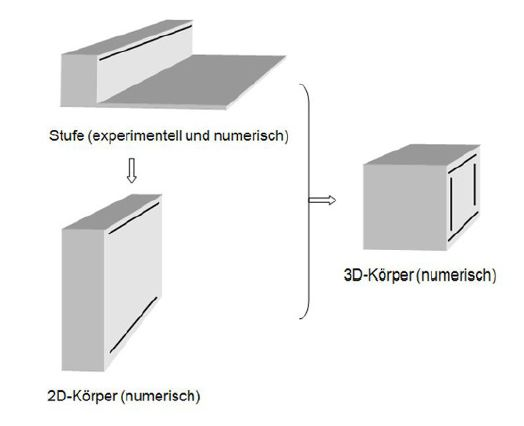
\includegraphics[width=0.5\textwidth]{KoerperGong.jpg}
	\caption{Modelle nach Gong \cite{Gong.2015}}
	\label{fig:Gong}
\end{figure}\\
Bei einer hochfrequenten Anregung kann die Bildung von Wirbeln unterdr"uckt werden. Dadurch wird der Druck hinter der Basis erh"oht und der Luftwiderstand des K"orpers sinkt.

%------------------------------------------------------------------------------------
Alle bisher vorgestellten Verfahren haben nur eine Steuerung des Vorgangs betrachtet. In \cite{Henning.2008} wird jetzt zus"atzlich eine Regelung des Mechanismuses der Str"omungsbeeinflussung eingef"uhrt. Dabei m"ochte man "au\ss{}ere St"orungen mit ber"ucksichtigen, die zum Beispiel sich gegenseitig beeinflussende Kraftfahrzeuge aufeinander haben.\\
Im Rahmen der Arbeit \cite{Henning.2008} wurden unterschiedliche K"orper "ahnlich zu denen in \abb{fig:Gong} analysiert.
%\begin{figure}[h]
%	\centering
%	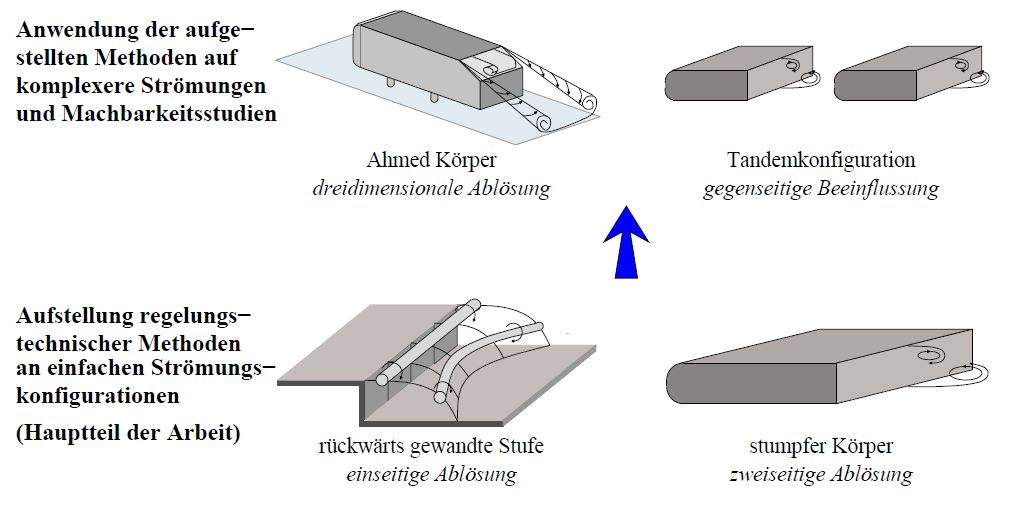
\includegraphics[width=0.8\textwidth]{KorperHenning.jpg}
%	\caption{betrachtete Modelle f"ur Auslegung der Regelung \cite{Henning.2008}}
%	\label{fig:Henning}
%\end{figure}\\
An der r"uck"arts gewandten Stufe wurde erfolgreich die Wideranlegel"ange "uber einen segmentierten Schlitz an der Stufenkante geregelt. Au\ss{}erdem konnte eine Unterdr"uckung von St"orungen erreicht werden. Das Ganze wurde "uber eine Robuste Regelung realisiert.\\
Am stumpfen K"orper wurde mit Hilfe einer Phasenregelung an Ober- und Unterseite eine Widerstandsreduzierung von bis zu 15\% erreicht.\\
Die Tandemkonfiguration (zwei K"orper hintereinander) wurde im Rahmen einer Machbarkeitsstudie \cite{Henning.2008} untersucht und f"ur zuk"unftige Arbeiten als sinnvoll betrachtet. Dabei geht es um die St"oreinfl"usse, die der erste K"orper auf den zweiten hat und wie dieser die St"orung "uber eine Regelung beseitigen kann, sodass auch beim zweiten K"orper eine Widerstandsreduzierung m"oglich ist.\\
Die Regelung stellt einen weiteren Schritt in Bezug auf eine Widerstandsreduktion von Stumpfk"orpern dar. Im Rahmen dieser Arbeit wird eine Regelung nicht mit betrachtet, da erst das neue Konzept untersucht werde muss. Dieses kann dann evtl. in Zukunft um eine Regelung erweitert werden.
